\chapter{Pengurutan}

\section{Kenapa belajar pengurutan?}
Manfaat mempelajari pengurutan dalam algoritma adalah sebagai berikut.
\begin{enumerate}
	\item Sering kali sebuah aplikasi memerlukan pengurutan, misalnya: aplikasi perbankan perlu mengurutkan data nasabah, aplikasi penjualan perlu mengurutkan catatan penjualan dan sebagainya.
	\item Banyak algoritma menggunakan pengurutan sebagai bagian atau fungsi dari algoritma tersebut. Sebagai contohnya, sebuah aplikasi pengolahan grafis tiga dimensi perlu melakukan pengurutan untuk menampilkan obyek secara betul dari atas sampai bawah (kedalaman).
	\item Dari algoritma pengurutan kita bisa mendapatkan banyak sekali teknik-teknik yang bermanfaat, bahkan banyak dari algoritma pengurutan yang sebenarnya sudah dikembangkan selama bertahun-tahun dan mengimplementasikan banyak teknik-teknik berguna yang bisa kita pelajari untuk digunakan di hal lain.
	\item Kita bisa menggunakan algoritma pengurutan sebagai salah satu tempat untuk mempelajari kompleksitas algoritma.
	\item Banyak bidang-bidang ilmu lain seperti misalnya basis data yang memerlukan algoritma pengurutan.
\end{enumerate}

\section{\textit{Bubble Sort}}
Algoritma \textit{Bubble Sort} merupakan algoritma pengurutan sederhana yang bekerja dengan cara membandingkan setiap elemen dari \textit{Array} dan menukarkan elemen-elemen tersebut. Algoritma \textit{Bubble Sort} bisa dilihat di Algoritma \ref{algo:bubble}.

Simulasi dari Algoritma \ref{algo:bubble} adalah sebagai berikut.
\begin{verbatim}
[4, 1, 3, 5, 6, 7, 2]

Loop:  1
A[ 0 ]( 4 )>= A[ 1 ]( 1 )= True
Tukar 4 dengan 1
[1, 4, 3, 5, 6, 7, 2]
A[ 0 ]( 1 )>= A[ 2 ]( 3 )= False
[1, 4, 3, 5, 6, 7, 2]
A[ 0 ]( 1 )>= A[ 3 ]( 5 )= False
[1, 4, 3, 5, 6, 7, 2]
A[ 0 ]( 1 )>= A[ 4 ]( 6 )= False
[1, 4, 3, 5, 6, 7, 2]
A[ 0 ]( 1 )>= A[ 5 ]( 7 )= False
[1, 4, 3, 5, 6, 7, 2]
A[ 0 ]( 1 )>= A[ 6 ]( 2 )= False
[1, 4, 3, 5, 6, 7, 2]

Loop:  2
A[ 1 ]( 4 )>= A[ 2 ]( 3 )= True
Tukar 4 dengan 3
[1, 3, 4, 5, 6, 7, 2]
A[ 1 ]( 3 )>= A[ 3 ]( 5 )= False
[1, 3, 4, 5, 6, 7, 2]
A[ 1 ]( 3 )>= A[ 4 ]( 6 )= False
[1, 3, 4, 5, 6, 7, 2]
A[ 1 ]( 3 )>= A[ 5 ]( 7 )= False
[1, 3, 4, 5, 6, 7, 2]
A[ 1 ]( 3 )>= A[ 6 ]( 2 )= True
Tukar 3 dengan 2
[1, 2, 4, 5, 6, 7, 3]

Loop:  3
A[ 2 ]( 4 )>= A[ 3 ]( 5 )= False
[1, 2, 4, 5, 6, 7, 3]
A[ 2 ]( 4 )>= A[ 4 ]( 6 )= False
[1, 2, 4, 5, 6, 7, 3]
A[ 2 ]( 4 )>= A[ 5 ]( 7 )= False
[1, 2, 4, 5, 6, 7, 3]
A[ 2 ]( 4 )>= A[ 6 ]( 3 )= True
Tukar 4 dengan 3
[1, 2, 3, 5, 6, 7, 4]

Loop:  4
A[ 3 ]( 5 )>= A[ 4 ]( 6 )= False
[1, 2, 3, 5, 6, 7, 4]
A[ 3 ]( 5 )>= A[ 5 ]( 7 )= False
[1, 2, 3, 5, 6, 7, 4]
A[ 3 ]( 5 )>= A[ 6 ]( 4 )= True
Tukar 5 dengan 4
[1, 2, 3, 4, 6, 7, 5]

Loop:  5
A[ 4 ]( 6 )>= A[ 5 ]( 7 )= False
[1, 2, 3, 4, 6, 7, 5]
A[ 4 ]( 6 )>= A[ 6 ]( 5 )= True
Tukar 6 dengan 5
[1, 2, 3, 4, 5, 7, 6]

Loop:  6
A[ 5 ]( 7 )>= A[ 6 ]( 6 )= True
Tukar 7 dengan 6
[1, 2, 3, 4, 5, 6, 7]
\end{verbatim}
\section{\textit{Insertion Sort}}

Algoritma \textit{Insertion Sort}\sidenote{\textit{Insertion Sort} mengurutkan \textbf{di tempat}: pengurutan terjadi di dalam \textit{array}} merupakan algoritma yang efisien untuk mengurutkan bilangan dalam jumlah yang kecil. Analogi \textit{Insertion Sort} mirip dengan cara seseorang mensortir kartu di tangannya dimana bisa dilihat di Gambar \ref{fig:InsertionSort}.

\begin{figure}%
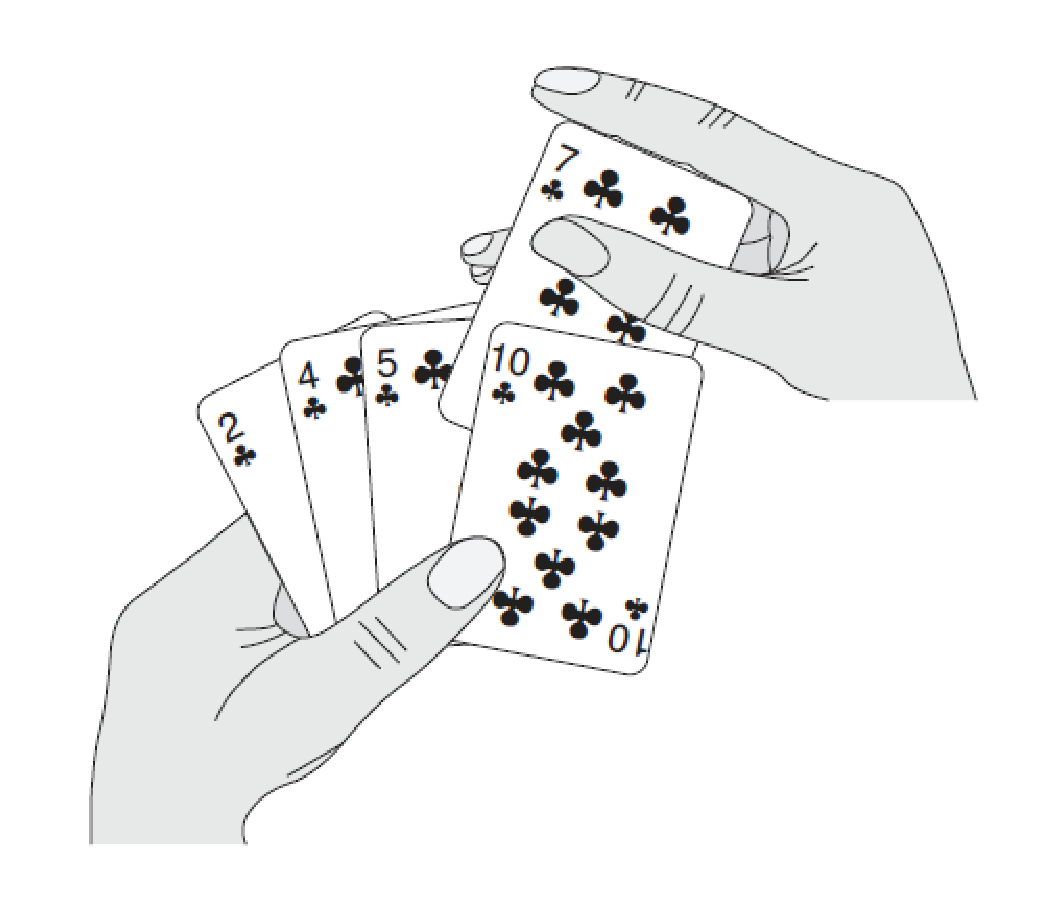
\includegraphics[scale=0.5]{fig/insertionSort.eps}%
\caption{Menyortir kartu di tangan}%
\label{fig:InsertionSort}%
\end{figure}


Algoritma \textit{Insertion Sort} bisa dilihat di Algoritma \ref{algo:insertion}. 
\begin{algorithm}[H]
	\caption{\textit{INSERTION-SORT(A)}}
	\label{algo:insertion}
	\begin{algorithmic}[1]
	\FOR {$j = 2$ to $A.length$}
		\STATE $key = A[j]$
		\STATE $i = j - 1$
		\WHILE {$i > 0$ and $A[i] > key$}
			\STATE $A[i+1] = A[i]$
			\STATE $i = i - 1$
		\ENDWHILE
		\STATE $A[i+1] = key$
	\ENDFOR
	\end{algorithmic}
\end{algorithm} 

\FloatBarrier
Cara kerja Algoritma \ref{algo:insertion} seperti illustrasi dibawah ini.
\begin{figure*}[htbp]%
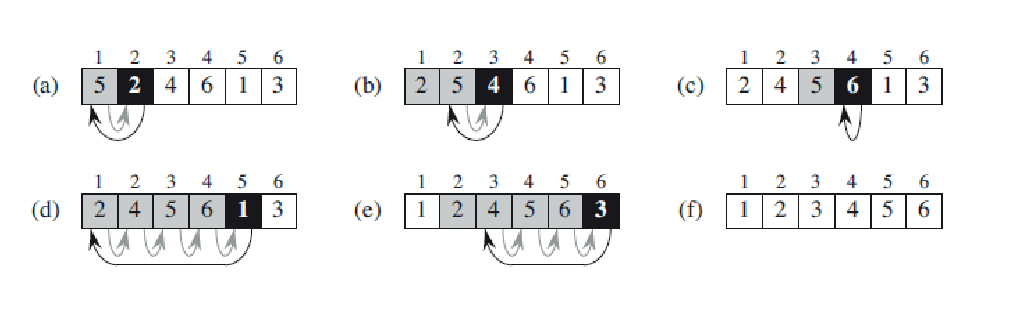
\includegraphics[scale=0.8]{fig/InsertionSortMethod}%
\caption{Cara kerja \textit{Insertion Sort}}%
\label{fig:caraKerjaInsertion}%
\end{figure*}
\FloatBarrier

Simulasi dari algoritma \textit{Insertion Sort} untuk \textit{array} A yang berisikan \{7,3,4,2,1\} adalah sebagai berikut.
\begin{verbatim}
Loop 1 , Key = 3 > [7, 3, 4, 2, 1] => [3, 7, 4, 2, 1]
Loop 2 , Key = 4 > [3, 7, 4, 2, 1] => [3, 4, 7, 2, 1]
Loop 3 , Key = 2 > [3, 4, 7, 2, 1] => [2, 3, 4, 7, 1]
Loop 4 , Key = 1 > [2, 3, 4, 7, 1] => [1, 2, 3, 4, 7]
\end{verbatim}

\begin{pemrograman}
Buatkan program python dari Algoritma \ref{algo:insertion}.
\end{pemrograman}

\begin{pemrograman}
\label{lat:cryptanalysis}
\textbf{Permasalahan Cryptanalysis}\\
\textit{Cryptanalysis} merupakan sebuah proses untuk memecahkan tulisan yang bersifat kriptografi. Proses tersebut melibatkan beberapa analisis statistika dari teks yang akan dipecahkan. Tugas anda adalah menuliskan sebuah program untuk melakukan analisis sederhana dari sebuah kalimat.\\
\textbf{Masukan}\\
Sebuah kalimat yang terdiri dari huruf A-Z, 0-9, spasi dan tanda baca lainnya.\\
\textbf{Keluaran}\\
Setiap baris terdiri dari bilangan A-Z dalam huruf kapital yang diikuti satu buah spasi dan bilangan integer positif yang menandakan jumlah huruf tersebut dalam kalimat masukan. Huruf kapital dan non kapital dalam kalimat masukan dianggap sama, bilangan dan spasi tidak dihitung. Keluarannya haruslah diurutkan berdasarkan alphabet yang duluan muncul. Hanya huruf yang muncul di kalimat masukan yang boleh ditampilkan dalam keluaran.\\
\begin{center}h
\textbf{Test Case 1}\\
\end{center}
\textbf{Masukan}\\
Hello, Selamat datang ke gubuk saya di alamat 45B!\\
\textbf{Keluaran}\\
A 9\\
B 2\\
D 2\\
E 3\\
G 2\\
H 1\\
I 1\\
K 2\\
L 4\\
M 2\\
N 1\\
O 1\\
S 2\\
T 3\\
Y 1\\
U 2\\
\begin{center}
\textbf{Test Case 2}\\
\end{center}
\textbf{Masukan}\\
Halo, no telepon saya adalah 543212\\
\textbf{Keluaran}\\
A 6\\
D 1\\
E 2\\
H 2\\
L 3\\
N 2\\
O 3\\
P 1\\
S 1\\
Y 1\\
T 1\\
\begin{center}
\textbf{Test Case 3}\\
\end{center}
\textbf{Masukan}\\
Apakah ini tuan Zainul?\\
\textbf{Keluaran}\\
A 5\\
H 1\\
I 3\\
K 1\\
L 1\\
N 3\\
P 1\\
T 1\\
Z 1\\
U 2\\
\end{pemrograman}